%-------------------------------------------------------
%    DOCUMENT CONFIGURATIONS
%-------------------------------------------------------

%-------------------------------------------------------
%    START OF ARCHITECTURE ANALYSE
%-------------------------------------------------------
\subsection{Architecture}
While doing research, the concept and based had to be pretty clear to help us focus on the right track. We then made an architecture for the project. Of course, this architecture is not definitive but contributes to the understanding of what we are trying to do. The latest global architecture version is found on figure ~\ref{fig:latest-architecture} in the annexes.

The main point of this architecture is to create a consensus-driven network. The nodes running on machines connected to the network are acting not more than clients.

paragraph{Consensus-driven} Working as a black-box, the goal of the is to applying the rules made by the identities. The security between the nodes is controlled by Overclouds, indeed, for client's point of view, they are talking with the network and not a particular node from the network. The network work is split into encrypted and distributed chunks to nodes. Note that the chunks are encrypted for the specific node as the keys are stored and owned by the consensus. Each node is participating by default to the network storage and computation power.

\paragraph{Storage} Controlled by the consensus and being the second part of Overclouds' black-box, storage allows the identities to save data into the distributed nodes of the network. Integrity checks are done by the consensus as multiple nodes are doing the same computation work and chunks storage (including redundancy).

\paragraph{Nodes} Considered as clients to the network, they have a trust level, which is stored on the network. This level increases over time with proof-of-participation and correct integrity checks. Identities' trust level is rising on the other hand for good behavior. This last point is described in the Big Picture chapter.

\begin{figure}[htpb]
\centering
\caption{Latest schematic architecture version seen from a User.
\label{fig:latest-schematic-architecture-user}} 
\begin{adjustbox}{center}
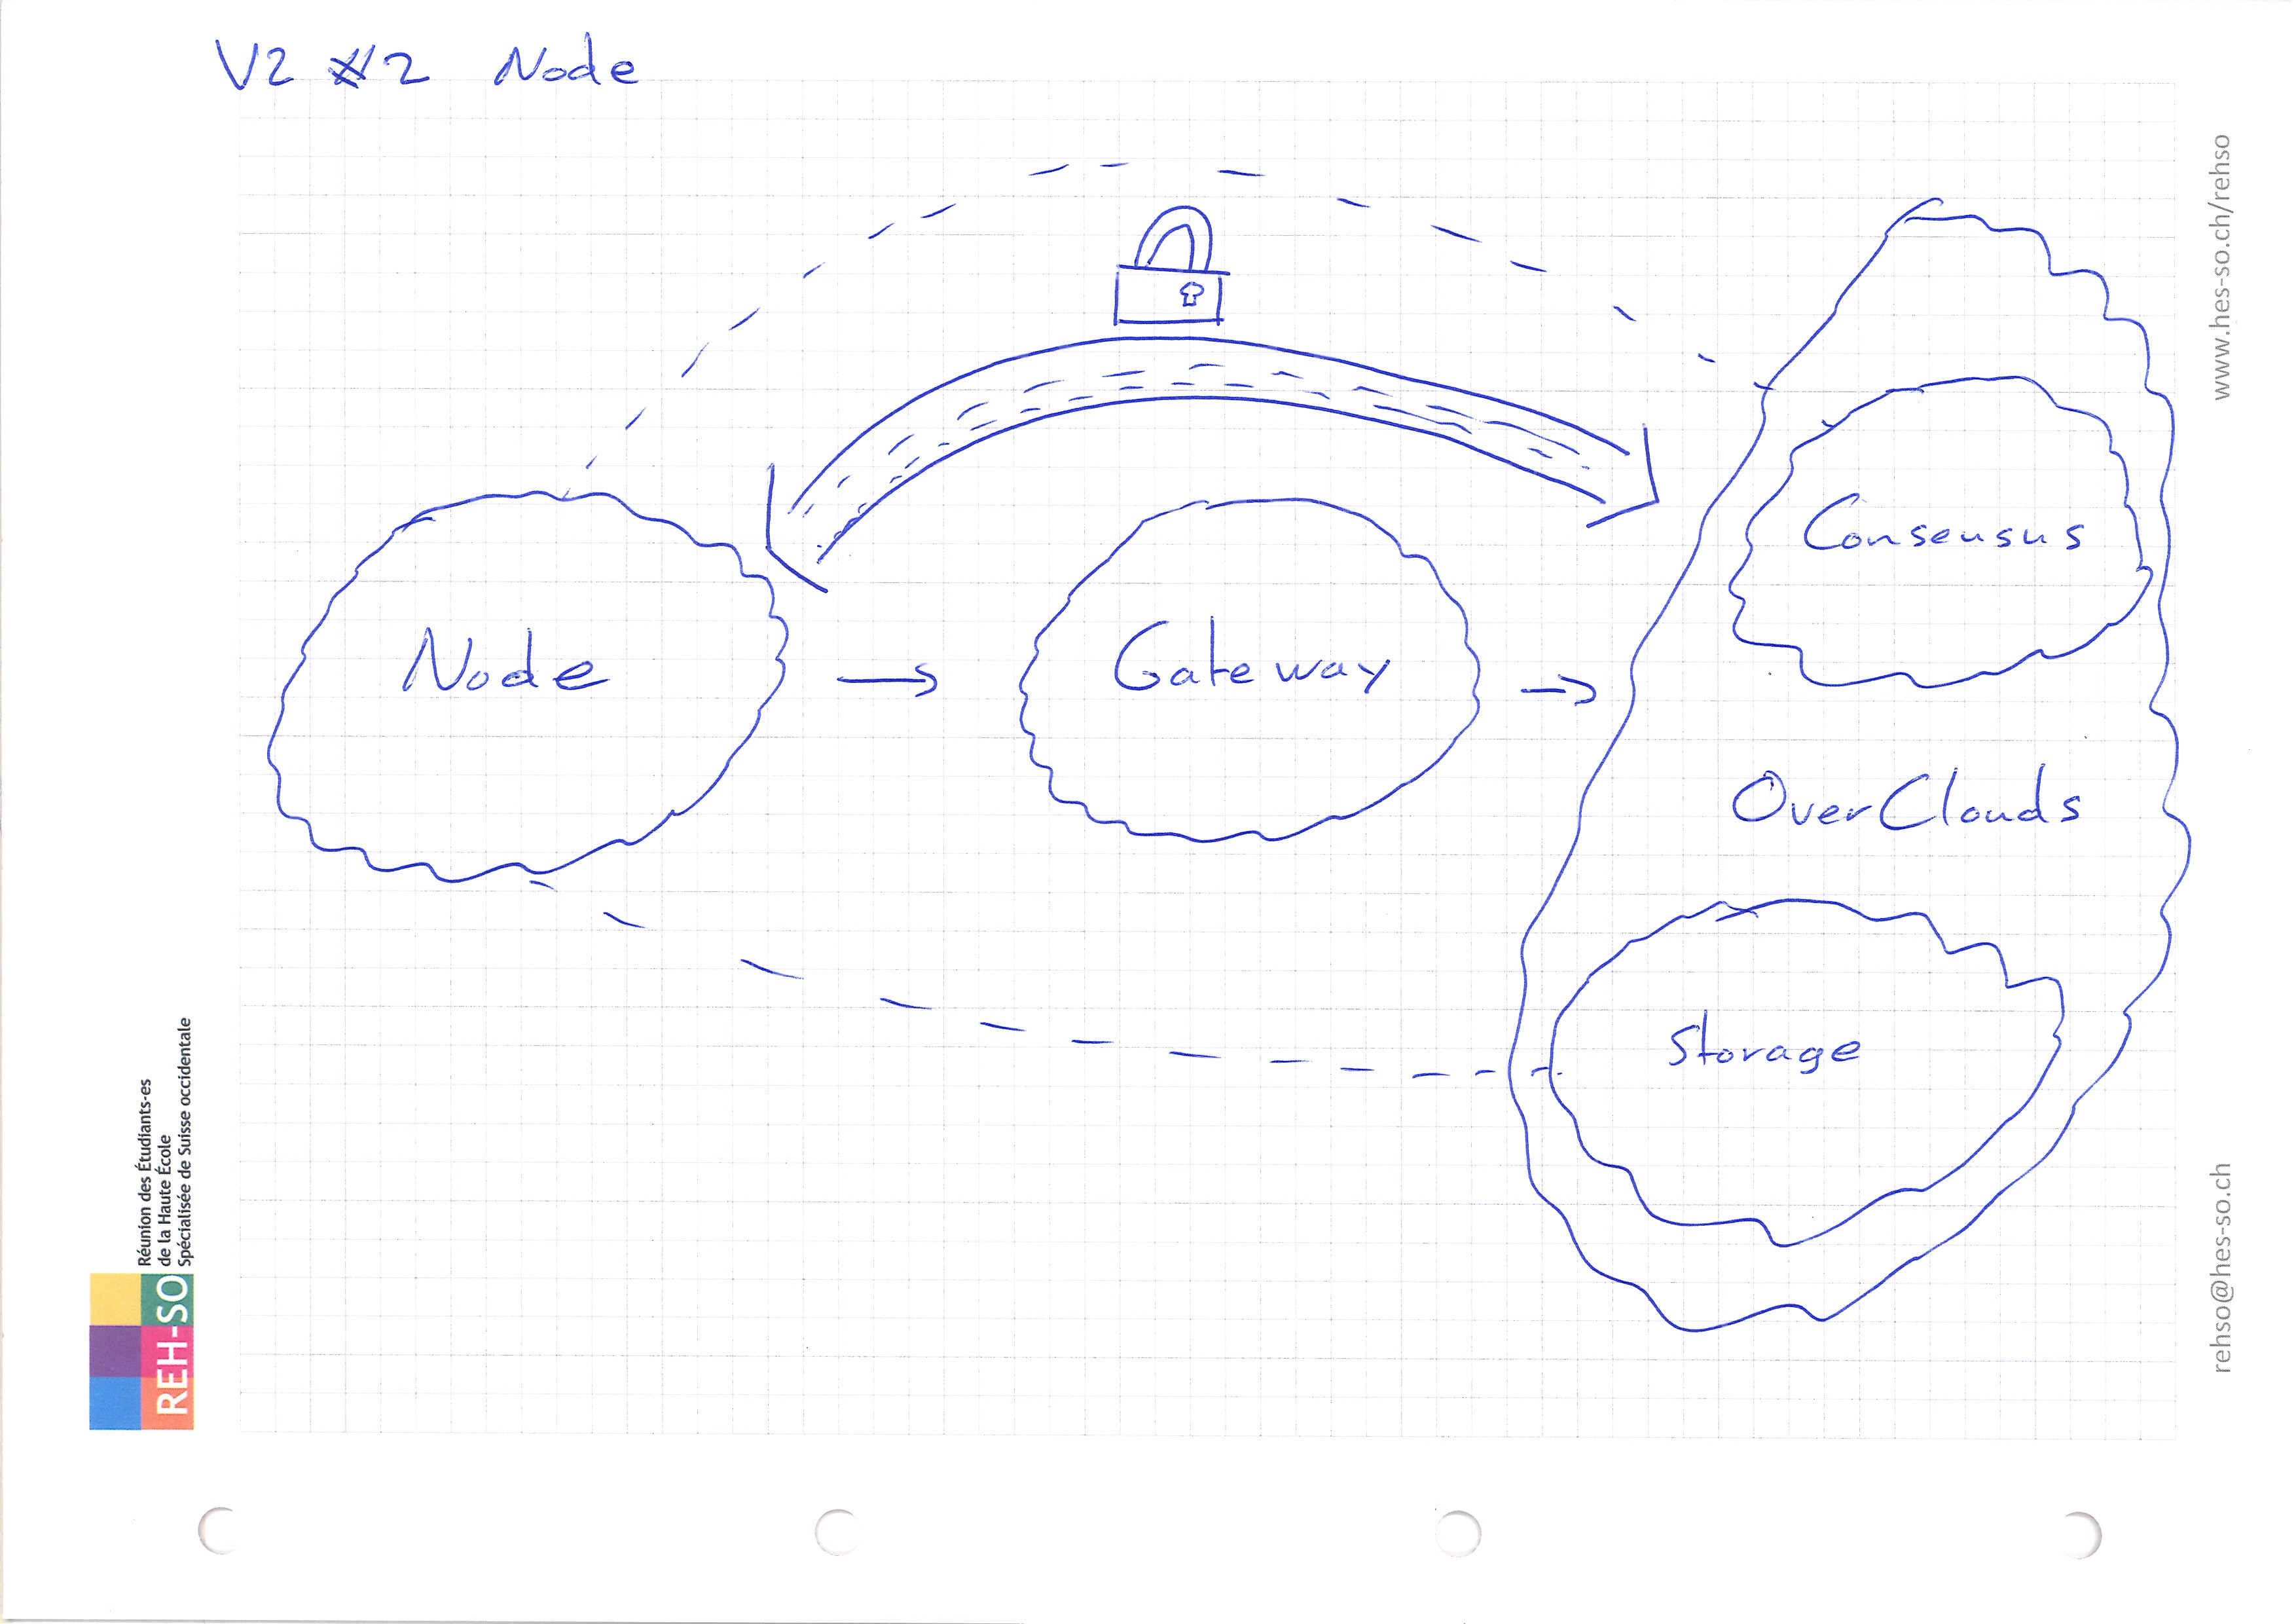
\includegraphics[scale=0.18]{annexes/concepts/Architecture-Draft-global-view-idea-2-node.jpeg}
\end{adjustbox} 
\end{figure}

\begin{figure}[htpb]
\centering
\caption{Latest schematic architecture version seen from a Node.
\label{fig:latest-schematic-architecture-node}} 
\begin{adjustbox}{center}
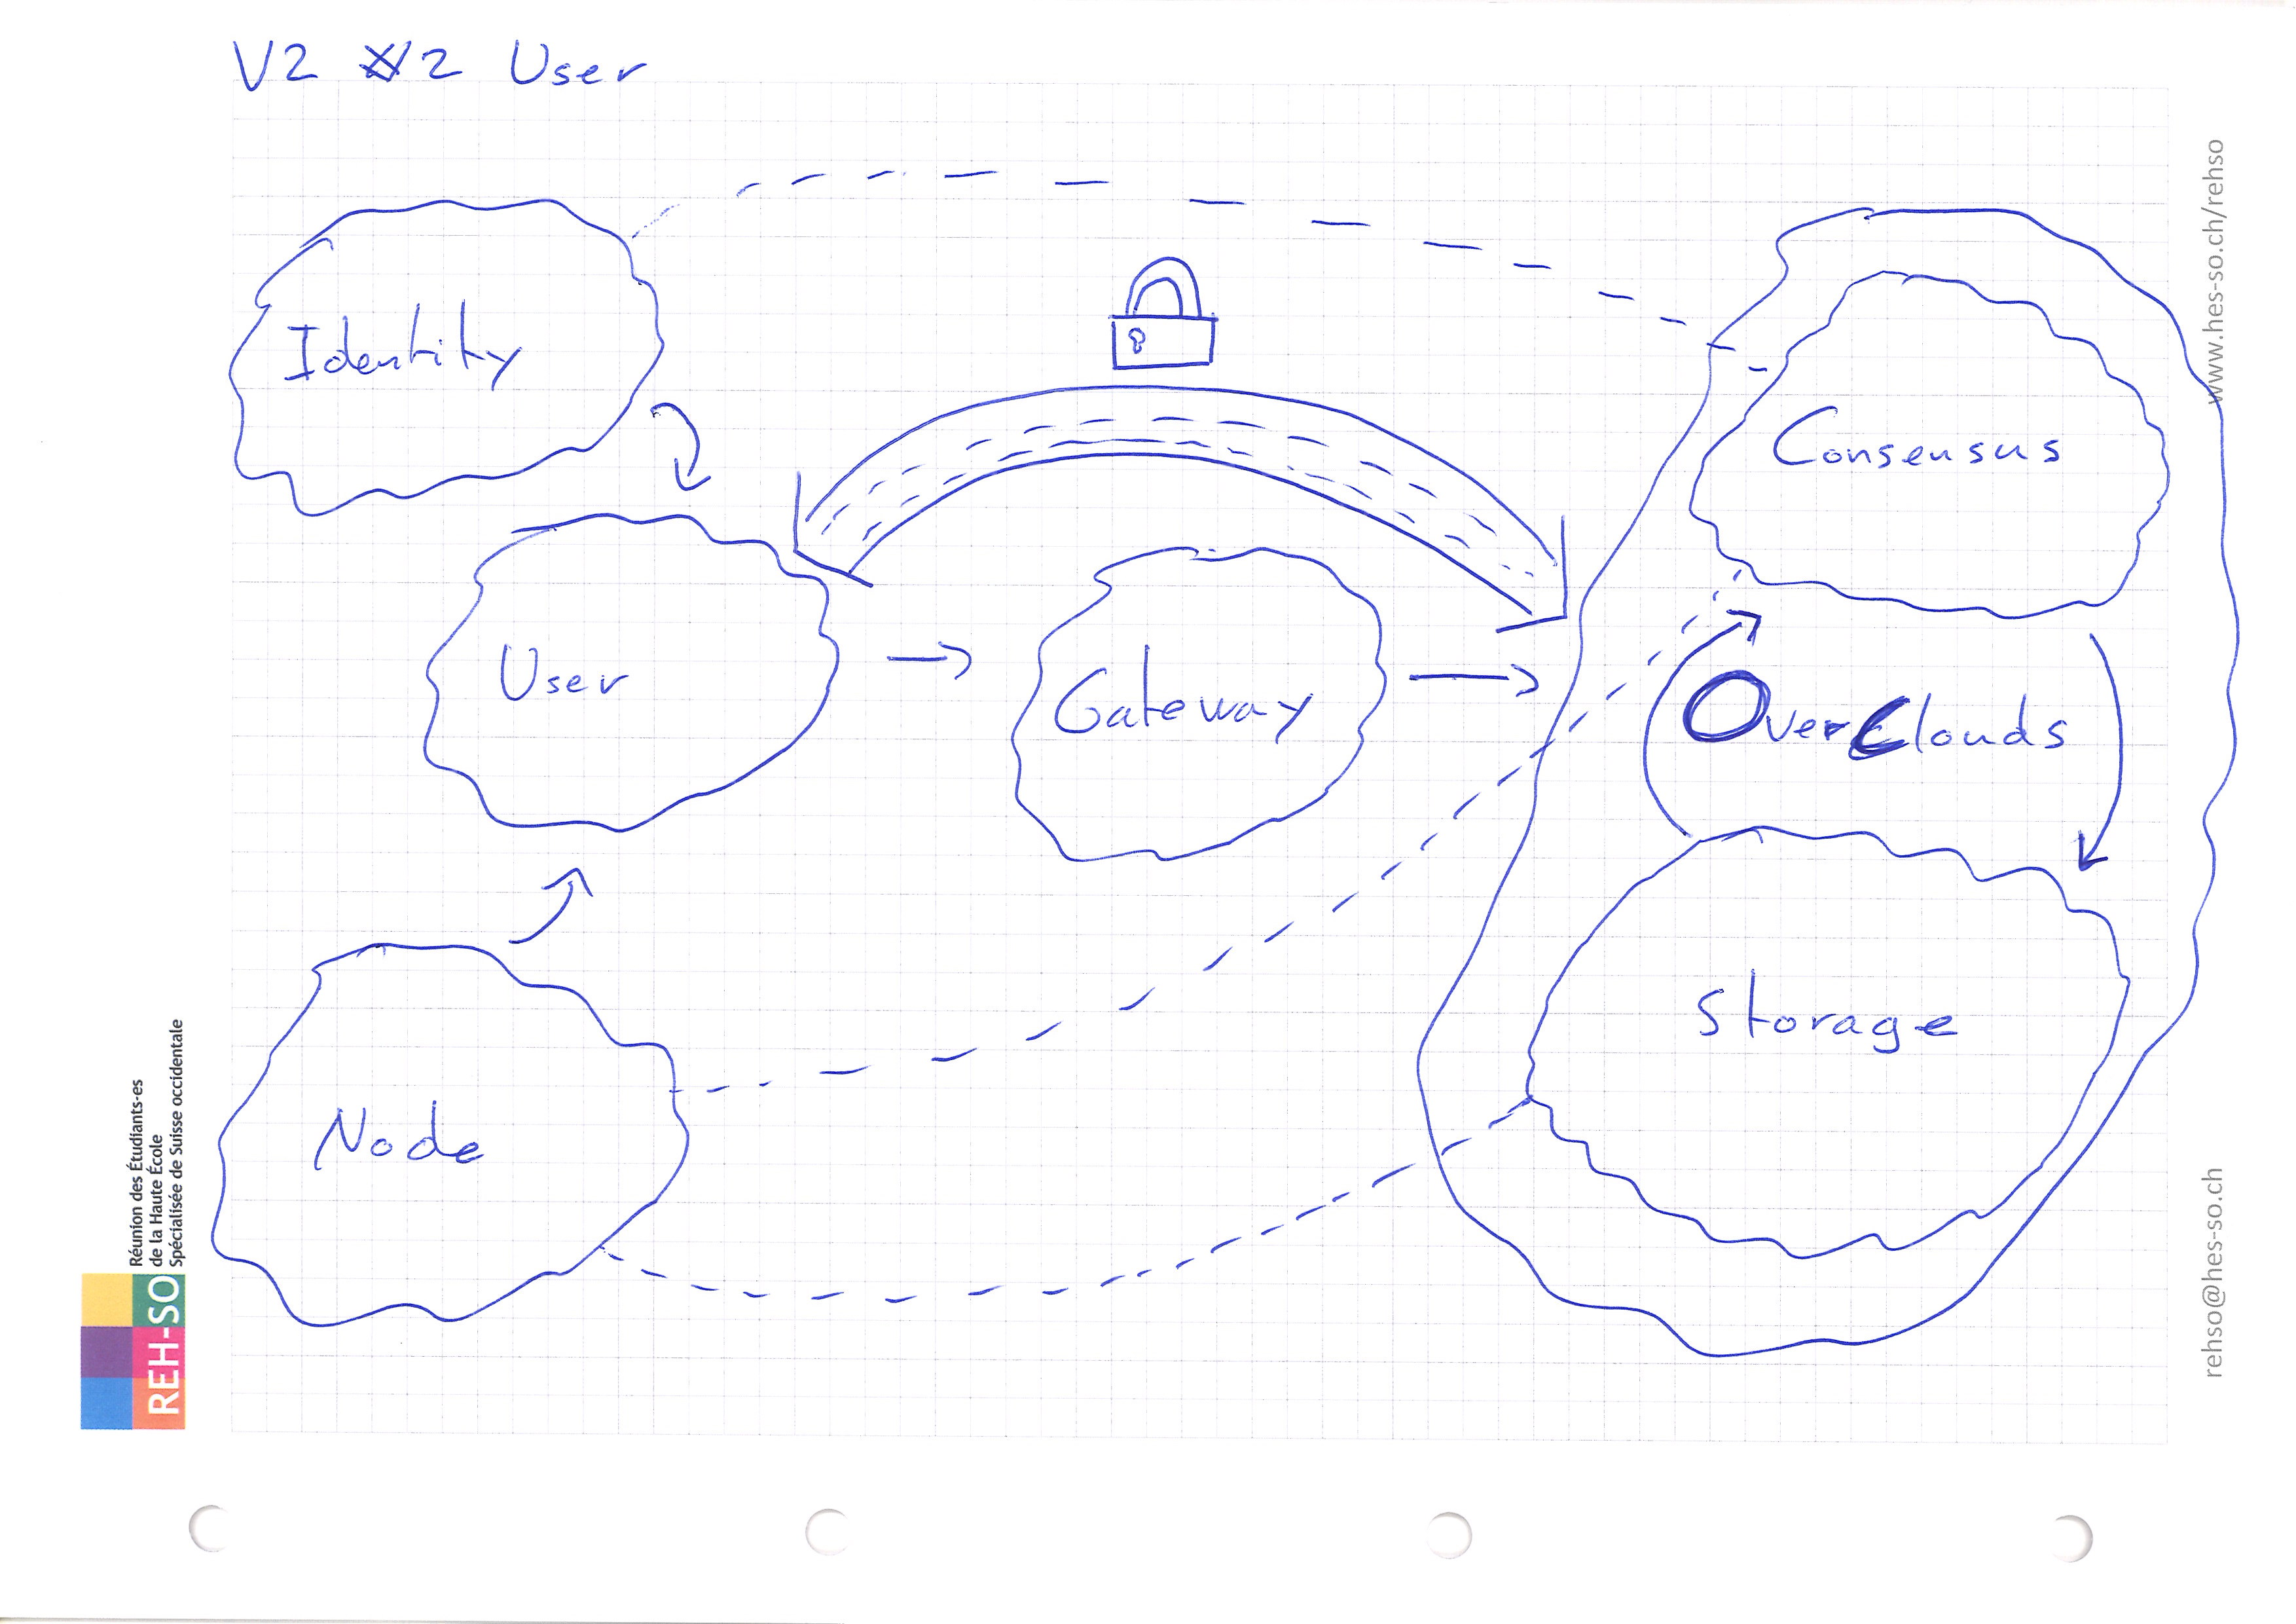
\includegraphics[scale=0.18]{annexes/concepts/Architecture-Draft-global-view-idea-2.jpeg}
\end{adjustbox} 
\end{figure}


%-------------------------------------------------------
%    END OF ARCHITECTURE ANALYSE
%-------------------------------------------------------